%% slides.tex — Slide thuyết trình (XeLaTeX + Beamer)
%% Biên dịch:  xelatex slides.tex   (chạy 2 lần để cập nhật mục lục)
%% Hình lấy từ ../../paper/figures/  (đường dẫn tương đối từ thư mục này)
\documentclass[aspectratio=169,11pt]{beamer}

\usepackage{fontspec}
\setmainfont{Arial}
\setsansfont{Arial}

\usepackage{graphicx}
\graphicspath{{../../paper/figures/}}
\usepackage{booktabs}
\usepackage{amsmath}

\usetheme{Madrid}
\useinnertheme{rounded}
\setbeamertemplate{navigation symbols}{}

% ── Bảng màu khớp với hình trong bài báo ────────────────────────────────────
\definecolor{vgreen}{HTML}{1E8449}
\definecolor{vpurple}{HTML}{6C3483}
\definecolor{vorange}{HTML}{B7460A}
\definecolor{vslate}{HTML}{2C3E50}
\definecolor{vlgray}{HTML}{7F8C8D}

\setbeamercolor{structure}{fg=vgreen}
\setbeamercolor{title}{fg=white}
\setbeamercolor{frametitle}{fg=white,bg=vgreen}
\setbeamercolor{alerted text}{fg=vorange}
\setbeamercolor{block title}{bg=vgreen!15,fg=vgreen}
\setbeamercolor{block body}{bg=vgreen!5}
\setbeamercolor{block title alerted}{bg=vorange!15,fg=vorange}
\setbeamercolor{block body alerted}{bg=vorange!5}
\setbeamerfont{frametitle}{series=\bfseries}
\setbeamertemplate{itemize item}{\color{vgreen}\textbullet}
\setbeamertemplate{itemize subitem}{\color{vlgray}--}

% footline gọn
\setbeamertemplate{footline}{%
  \leavevmode\hbox{%
  \begin{beamercolorbox}[wd=.78\paperwidth,ht=2.4ex,dp=1.2ex,leftskip=1em]{author in head/foot}%
    \usebeamerfont{author in head/foot}DyAM + OvO + NLP \,—\, Dự đoán đáp ứng ICI trong NSCLC%
  \end{beamercolorbox}%
  \begin{beamercolorbox}[wd=.22\paperwidth,ht=2.4ex,dp=1.2ex,rightskip=1em]{title in head/foot}%
    \hfill\insertframenumber\,/\,\inserttotalframenumber%
  \end{beamercolorbox}}%
}

\title[NLP-Augmented Multimodal Attention]{Tích hợp đa phương thức dựa trên cơ chế Attention\\ tăng cường NLP để dự đoán đáp ứng miễn dịch\\ trong ung thư phổi không tế bào nhỏ}
\subtitle{\small Phát triển trên nền tảng DyAM (Vanguri et al., \textit{Nature Cancer} 2022)}
\author[Học viên]{Học viên thực hiện}
\institute[]{\small Người hướng dẫn: [Tên GVHD] \quad•\quad [Đơn vị]}
\date{\today}

\begin{document}

% ═══════════════════════════════════════════════════════════════════════════
\begin{frame}[plain]
  \titlepage
\end{frame}

% ───────────────────────────────────────────────────────────────────────────
\begin{frame}{Nội dung trình bày}
  \tableofcontents
\end{frame}

% ═══════════════════════════════════════════════════════════════════════════
\section{Đặt vấn đề}

\begin{frame}{Bài toán lâm sàng}
  \begin{itemize}
    \item Ung thư phổi là nguyên nhân tử vong do ung thư \alert{hàng đầu} thế giới; NSCLC chiếm \alert{$\approx$85\%} số ca.
    \item Liệu pháp miễn dịch ICI (ức chế trục PD-1/PD-L1) tạo \alert{đột phá} điều trị, đáp ứng bền vững ở một nhóm bệnh nhân.
    \item \textbf{Nhưng chỉ 20–30\% bệnh nhân đáp ứng} — phần lớn kháng thuốc nguyên phát hoặc mắc phải.
  \end{itemize}
  \vfill
  \begin{block}{Nhu cầu lâm sàng}
    Dự đoán \textbf{trước điều trị} bệnh nhân nào có khả năng đáp ứng $\Rightarrow$ ưu tiên đúng người, tránh điều trị tốn kém và độc tính cho người ít khả năng đáp ứng.
  \end{block}
\end{frame}

\begin{frame}{Hạn chế của biomarker hiện tại}
  \begin{itemize}
    \item Hai biomarker phổ biến: \textbf{PD-L1 TPS} và \textbf{TMB} — khả năng phân biệt còn hạn chế.
    \begin{itemize}
      \item PD-L1: không đồng nhất về không gian, phụ thuộc loại xét nghiệm.
      \item TMB đơn lẻ: chỉ phân biệt ở mức trung bình.
    \end{itemize}
    \item[$\Rightarrow$] Xu hướng \alert{tích hợp đa phương thức}: radiomics (CT) + bệnh học (mô) + genomics + lâm sàng.
  \end{itemize}
  \vfill
  \begin{block}{Thách thức của hướng đa phương thức}
    (1) Gán trọng số cho các phương thức có \textbf{độ tin cậy khác nhau}; \quad
    (2) Xử lý \textbf{dữ liệu thiếu} mà không loại bỏ bệnh nhân.
  \end{block}
\end{frame}

\begin{frame}{Mô hình nền DyAM \& khoảng trống nghiên cứu}
  \textbf{DyAM} (Vanguri 2022): attention học theo \textit{từng bệnh nhân}, tự gán trọng số mỗi phương thức, xử lý dữ liệu thiếu bằng \textit{masking}.
  \vfill
  \begin{alertblock}{Hai khoảng trống chưa giải quyết}
    \begin{enumerate}
      \item \textbf{Biểu diễn biến lâm sàng:} DyAM dùng \textit{số thô} $\rightarrow$ bỏ mất quan hệ giữa các biến (tuổi cao + albumin thấp + ECOG kém).
      \item \textbf{Dạng attention:} DyAM chỉ dùng attention \textit{hợp tác} (cooperative) $\rightarrow$ ngầm giả định mọi phương thức bổ sung, cộng gộp.
    \end{enumerate}
  \end{alertblock}
\end{frame}

\begin{frame}{Mục tiêu \& đóng góp}
  \begin{block}{Đóng góp 1 — OvO competitive attention}
    Cơ chế attention \textbf{cạnh tranh} (one-vs-others); so sánh với attention hợp tác gốc trên \textbf{20 tổ hợp} phương thức.
  \end{block}
  \begin{block}{Đóng góp 2 — NLP encoding}
    Chuyển \textbf{13 biến lâm sàng số} $\rightarrow$ câu tiếng Anh $\rightarrow$ embedding bằng sentence-transformer (MiniLM-L6-v2).
  \end{block}
  \vfill
  \footnotesize Đánh giá trên \textbf{cả hai trục}: phân loại nhị phân (AUC) \textbf{và} phân tích sống còn (Cox, C-index, Kaplan–Meier). Cohort khám phá: \textbf{247 bệnh nhân} NSCLC điều trị ICI.
\end{frame}

% ═══════════════════════════════════════════════════════════════════════════
\section{Phương pháp}

\begin{frame}{Tổng quan thiết kế nghiên cứu}
  \centering
  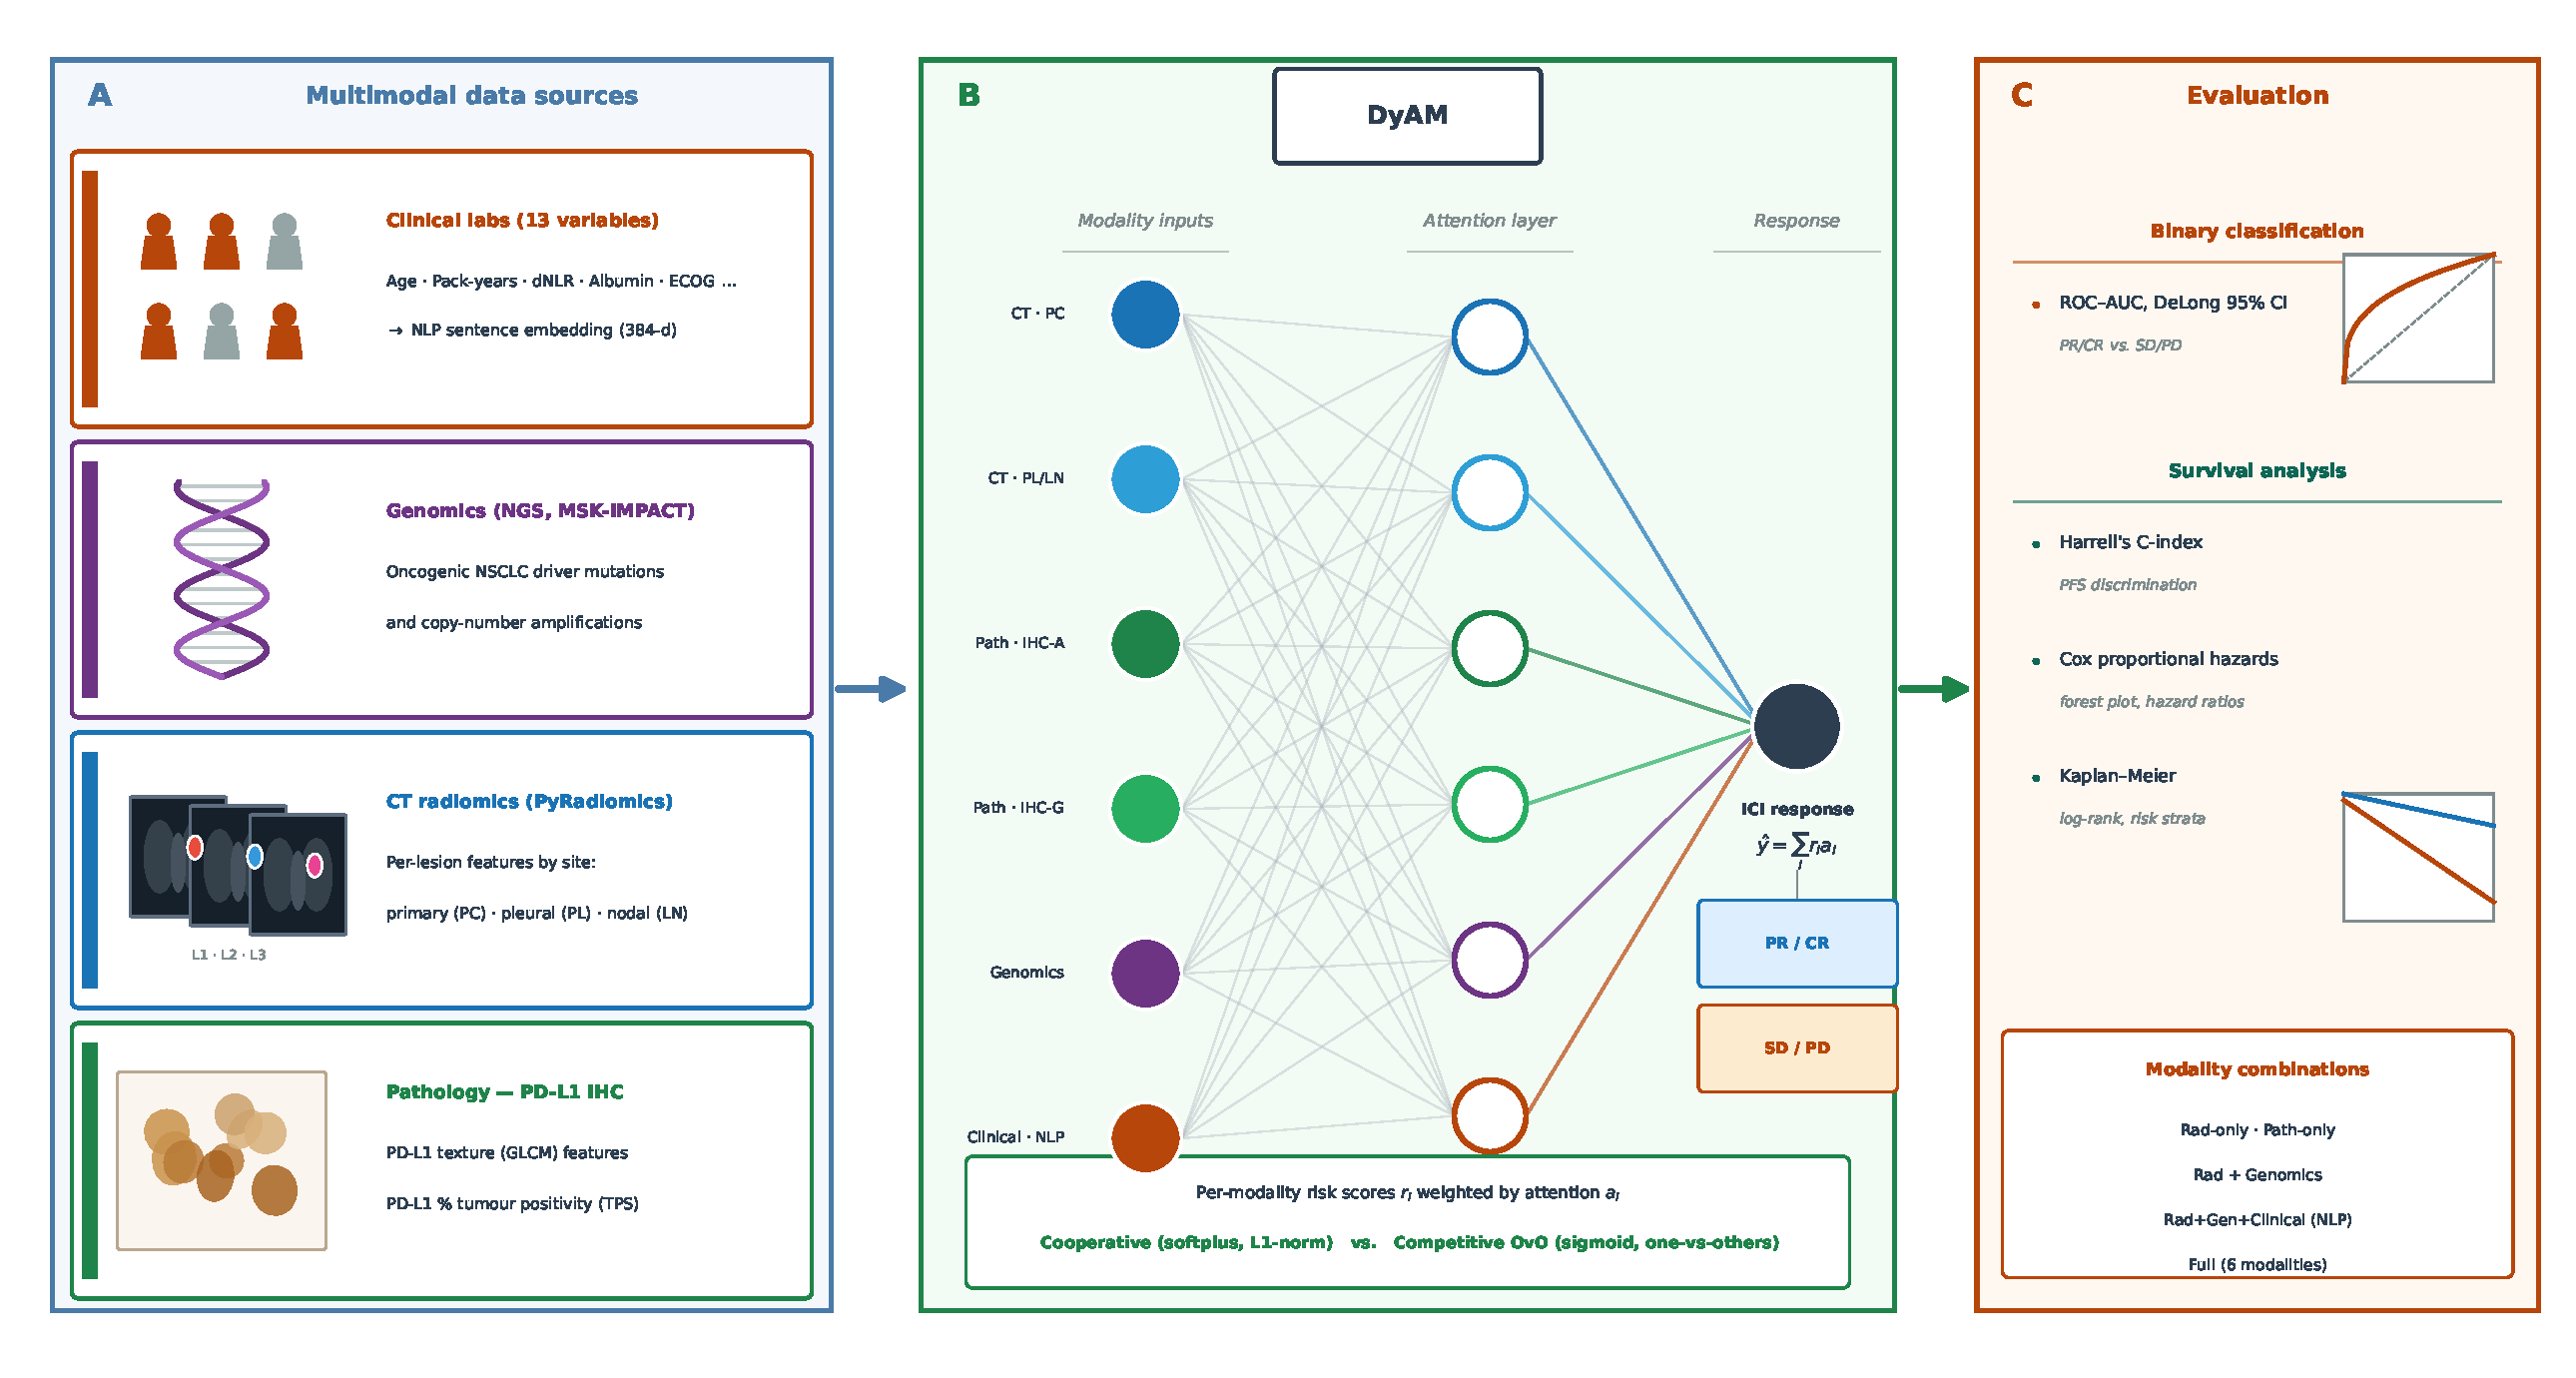
\includegraphics[width=0.96\textwidth]{fig1_overview.pdf}
  \par\vspace{0.3em}
  \footnotesize (A) Nguồn dữ liệu \;•\; (B) Kiến trúc DyAM: risk score $+$ attention \;•\; (C) Đánh giá AUC \& sống còn
\end{frame}

\begin{frame}{Hai cơ chế Attention --- điểm cốt lõi}
  \begin{columns}[T]
    \begin{column}{0.62\textwidth}
      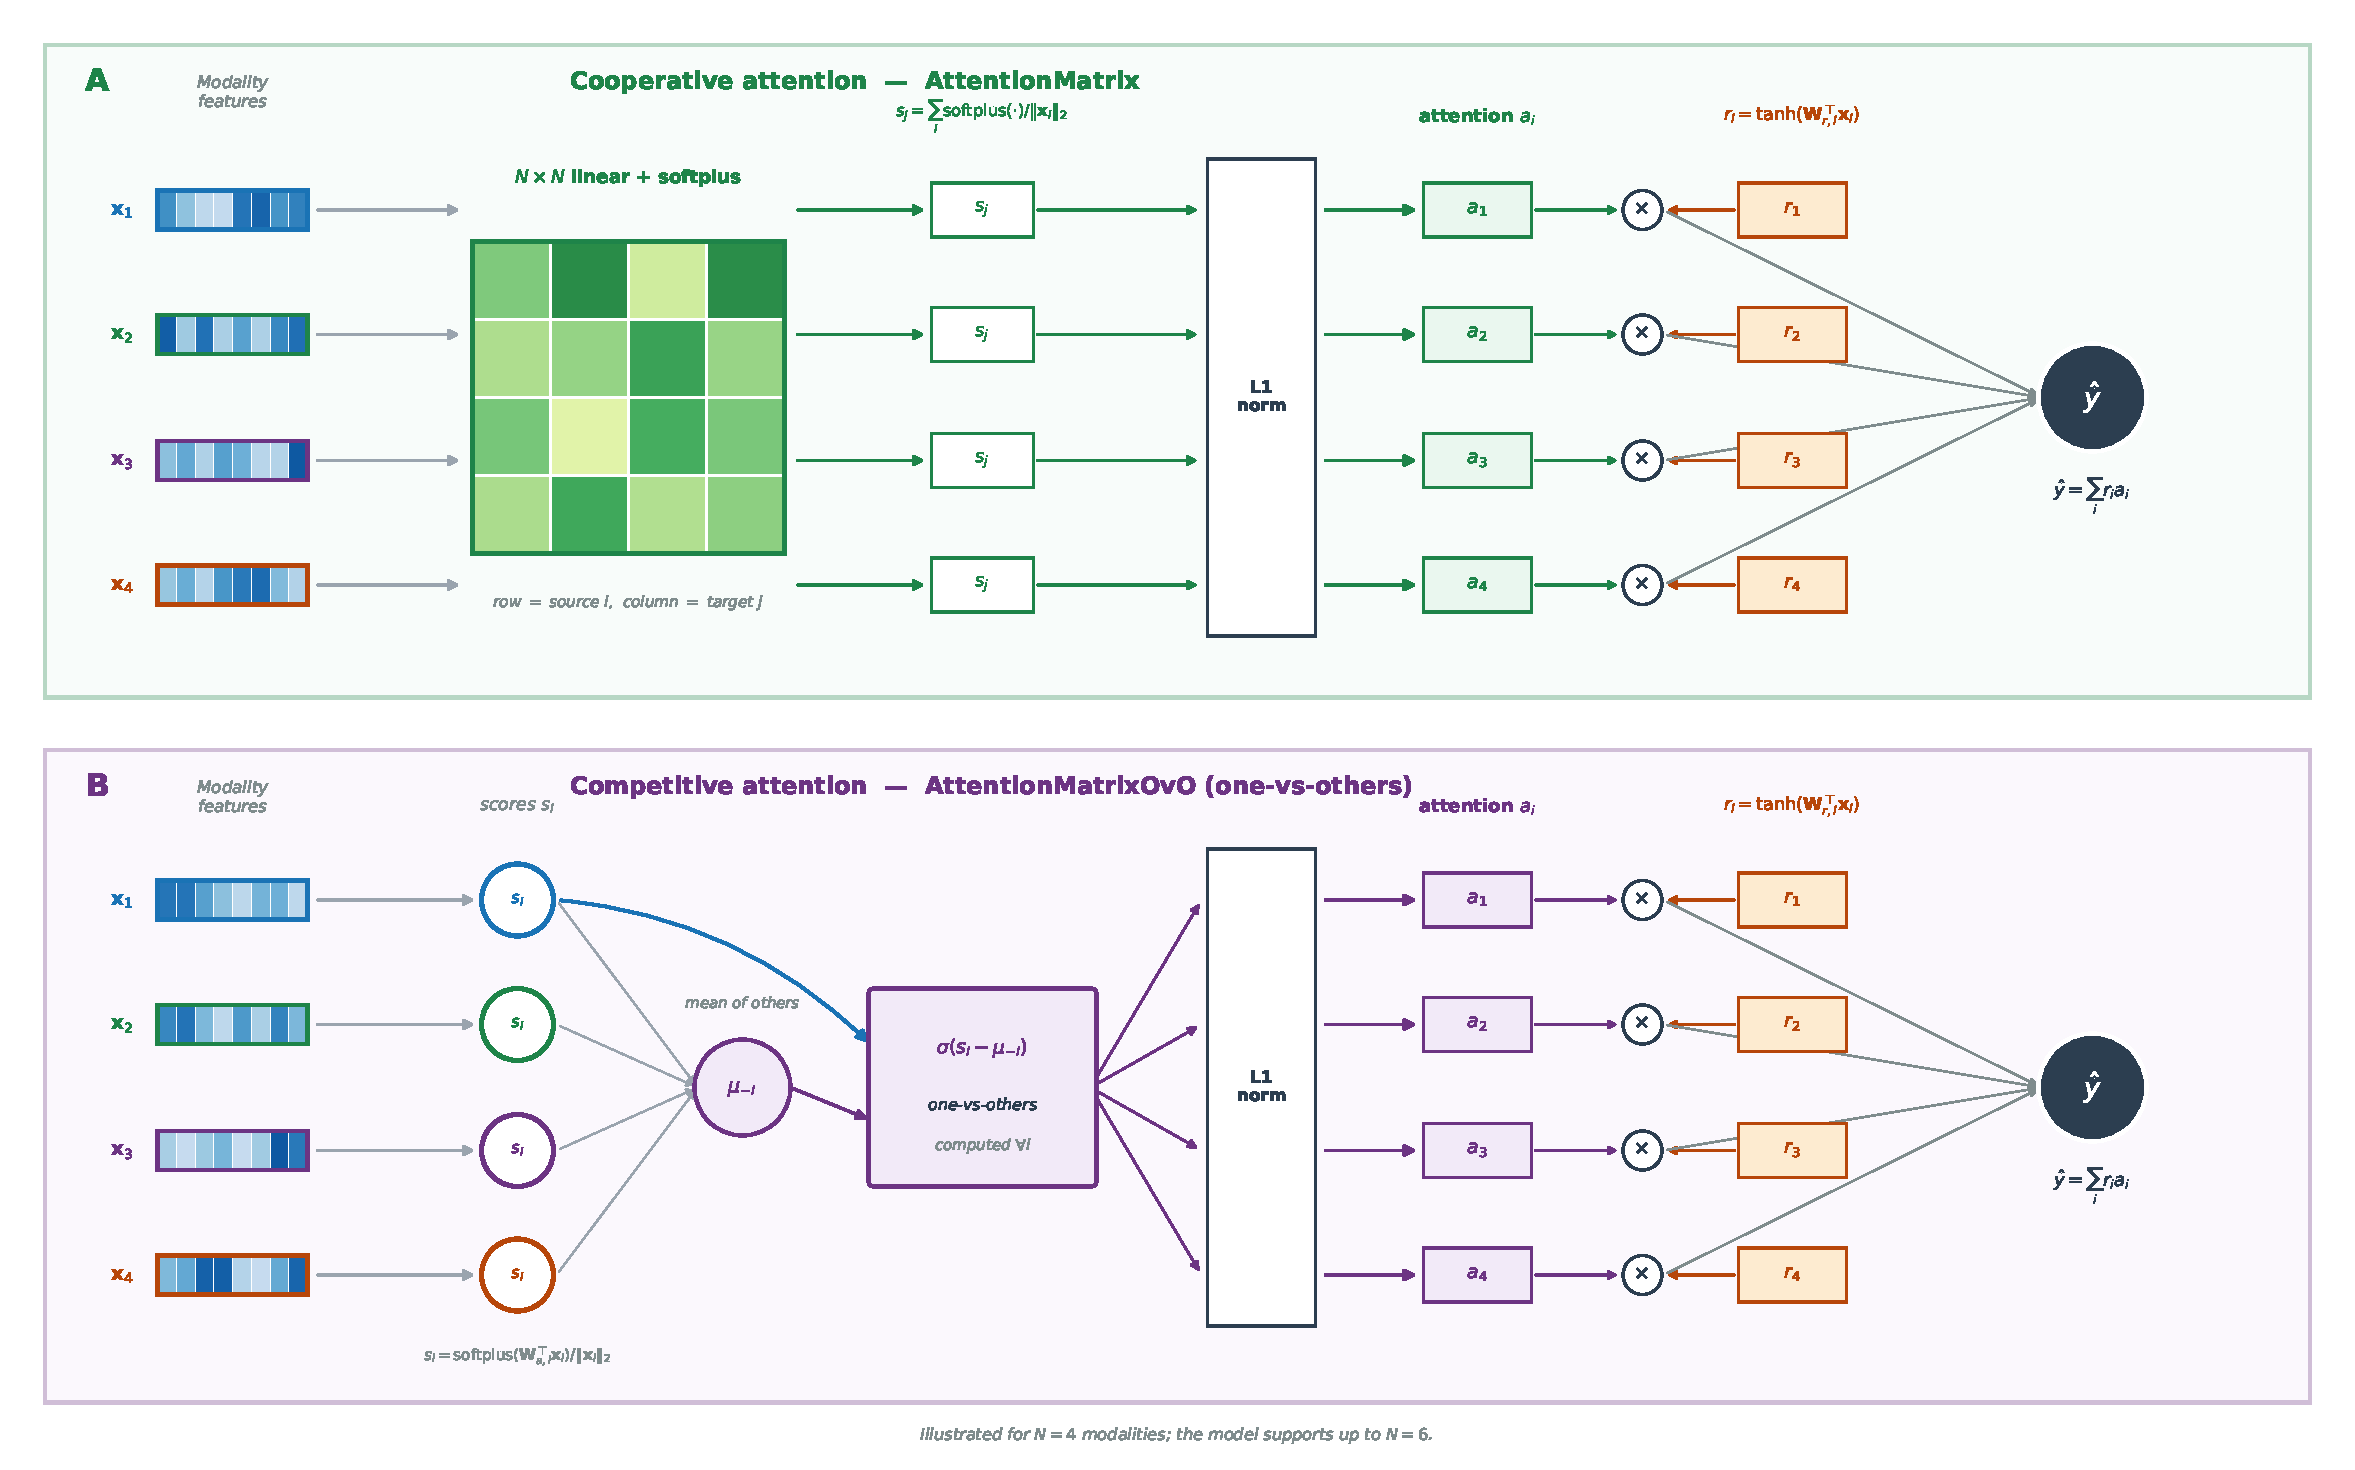
\includegraphics[width=\textwidth]{fig_attention_arch.pdf}
    \end{column}
    \begin{column}{0.38\textwidth}
      \scriptsize
      Cả hai: $r_i=\tanh(\mathbf{W}_{r,i}^{\top}\mathbf{x}_i)$,\quad $\hat{y}=\sum_i r_i a_i$.
      \vspace{0.6em}
      \begin{block}{(A) Cooperative}
        Ma trận $N\times N$ + softplus $\rightarrow$ L1-norm. Các phương thức \textbf{chia sẻ ngân sách} (tổng $=1$).
      \end{block}
      \begin{block}{(B) Competitive OvO}
        $\sigma(s_i-\mu_{-i})$: mỗi phương thức so với \textbf{trung bình các phương thức còn lại}. Trọng số \textbf{độc lập}, kiểu ``best-of''.
      \end{block}
    \end{column}
  \end{columns}
\end{frame}

\begin{frame}{Đóng góp 2: NLP encoding cho biến lâm sàng}
  \centering
  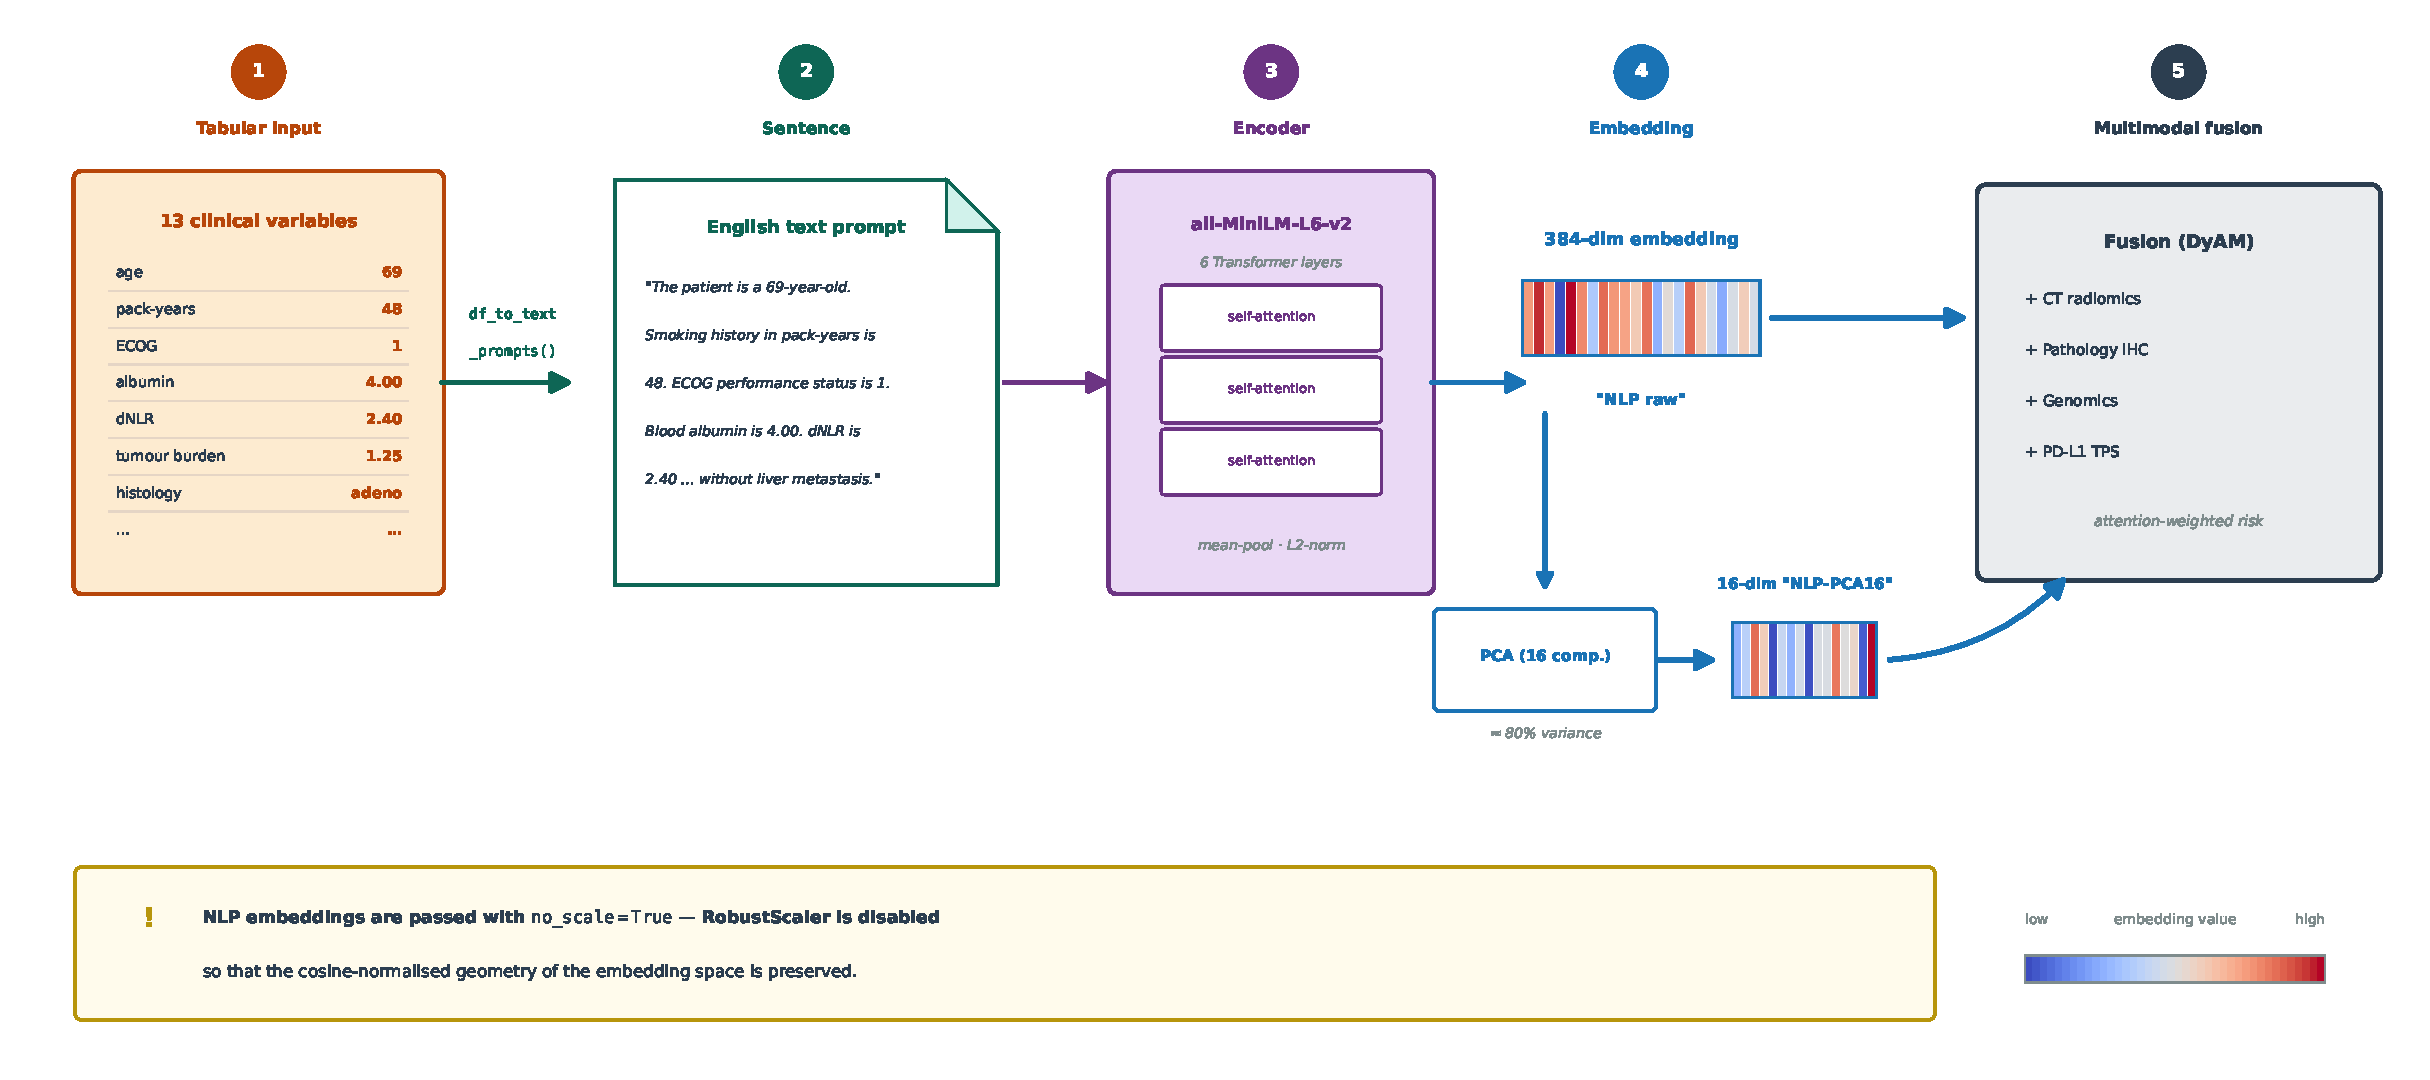
\includegraphics[width=0.98\textwidth]{fig2_nlp_pipeline.pdf}
  \par\vspace{0.2em}
  \footnotesize
  13 biến số $\rightarrow$ câu tiếng Anh $\rightarrow$ MiniLM-L6-v2 $\rightarrow$ embedding \textbf{384-d} (``NLP raw'') / PCA \textbf{16-d}.\\
  \alert{Quan trọng:} \texttt{no\_scale=True} để giữ hình học cosine của embedding. Không cần fine-tune, $<$1s/bệnh nhân trên CPU.
\end{frame}

\begin{frame}{Dữ liệu \& phương pháp đánh giá}
  \begin{columns}[T]
    \begin{column}{0.5\textwidth}
      \textbf{Dữ liệu \& huấn luyện}
      \begin{itemize}
        \item Cohort khám phá: \textbf{247 BN} NSCLC
        \item Nhãn: đáp ứng (PR/CR) vs không (SD/PD); mất cân bằng \textbf{$\approx$1:3}
        \item BCE loss + cân bằng lớp tự động; Adam; \textbf{10-fold CV}
      \end{itemize}
    \end{column}
    \begin{column}{0.5\textwidth}
      \textbf{Đánh giá}
      \begin{itemize}
        \item Nhị phân: \textbf{AUC-ROC} + CI DeLong 95\%
        \item Sống còn (PFS): \textbf{Cox HR}, time-dependent AUC, \textbf{C-index}, IBS, \textbf{Kaplan–Meier} log-rank
      \end{itemize}
    \end{column}
  \end{columns}
  \vfill
  \begin{block}{Điểm nhấn}
    Đánh giá cả \textit{predictive} (đáp ứng) lẫn \textit{prognostic} (sống còn) $\rightarrow$ về sau cho một phát hiện thú vị.
  \end{block}
\end{frame}

% ═══════════════════════════════════════════════════════════════════════════
\section{Kết quả}

\begin{frame}{KQ1: Đa phương thức vượt đơn phương thức}
  \begin{itemize}
    \item Đơn phương thức (logistic regression):
    \begin{itemize}
      \item AUC 0,570 (lâm sàng) • 0,640 (radiomics) • 0,650 (genomics) • 0,729 (PD-L1)
    \end{itemize}
  \end{itemize}
  \vfill
  \begin{alertblock}{DyAM tích hợp 4 phương thức: AUC $= 0{,}784$ [0,717–0,850]}
    Tích hợp đa phương thức là \textbf{động lực chính} của hiệu năng, vượt xa mọi phương thức đơn lẻ.
  \end{alertblock}
\end{frame}

\begin{frame}{KQ2: OvO attention --- lợi ích phụ thuộc ngữ cảnh}
  \begin{itemize}
    \item 20 tổ hợp: OvO thắng \textbf{7}, Original thắng \textbf{9}, hòa 4.
    \item \textbf{2 phương thức:} OvO tốt hơn 3/6 — lớn nhất PDL1+Gen \alert{$+3{,}27\%$}, Rad+Gen $+2{,}23\%$.
    \item \textbf{$\geq$3 phương thức:} Original tốt hơn 6/10 (nhất là khi có IHC-G / lâm sàng).
  \end{itemize}
  \vfill
  \begin{alertblock}{Cấu hình tốt nhất toàn bộ: OvO Rad+IHC-G+Gen+PDL1 — AUC $=0{,}800$ [0,739–0,862]}
    OvO hợp với phương thức \textbf{trùng lặp} (chọn ``best-of''); cooperative hợp khi nhiều phương thức \textbf{bổ sung}.
  \end{alertblock}
\end{frame}

\begin{frame}{KQ3: NLP cải thiện AUC ổn định}
  \begin{columns}[c]
    \begin{column}{0.5\textwidth}
      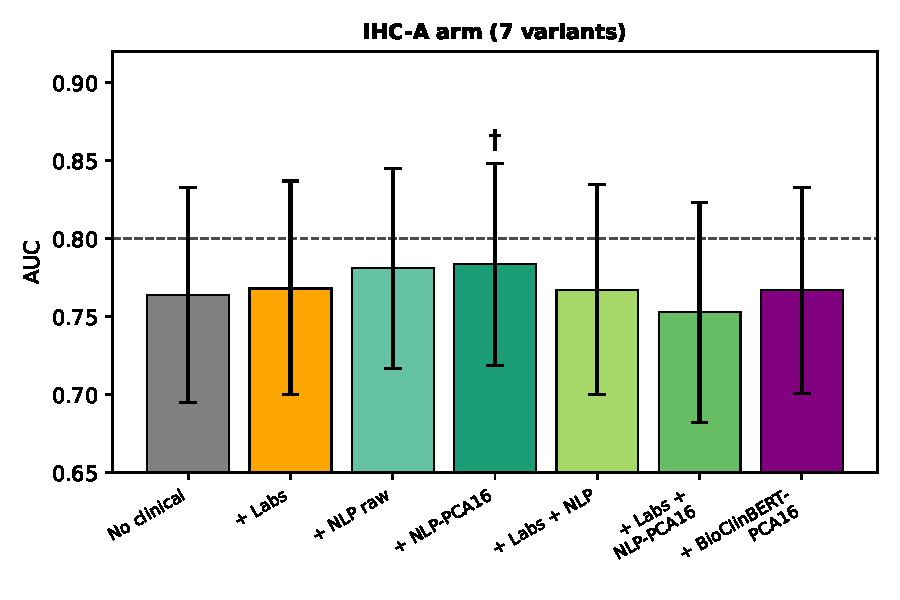
\includegraphics[width=\textwidth]{fig3a_auc_ihca.pdf}
    \end{column}
    \begin{column}{0.5\textwidth}
      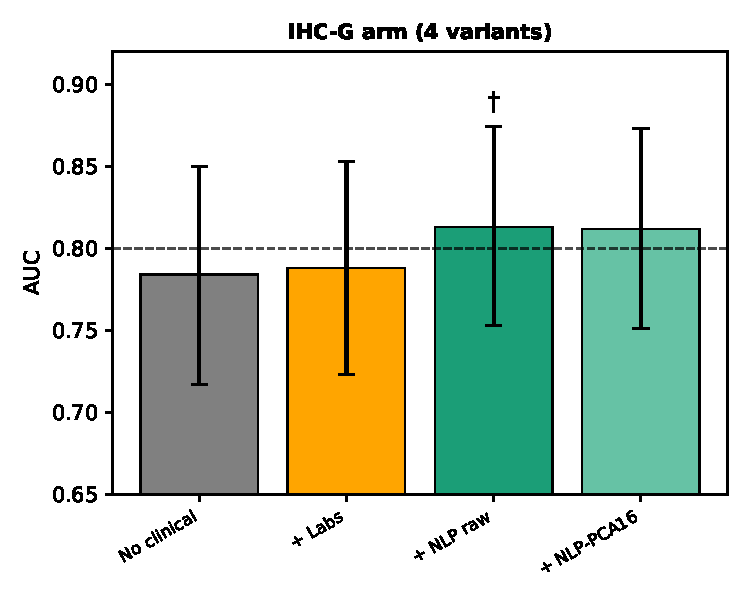
\includegraphics[width=\textwidth]{fig3b_auc_ihcg.pdf}
    \end{column}
  \end{columns}
  \vspace{0.2em}
  \footnotesize
  \begin{itemize}
    \item IHC-A: \textbf{NLP-PCA16} tốt nhất (AUC 0,784; $\Delta=+0{,}020$) vs $+0{,}004$ cho số thô.
    \item IHC-G: \textbf{NLP raw} tốt nhất (AUC \alert{0,813}; $\Delta=+0{,}030$). Cải thiện \textbf{nhất quán}, nhưng CI còn chồng lấn.
    \item BioClinBERT (chuyên y khoa) \textbf{kém hơn} MiniLM tổng quát.
  \end{itemize}
\end{frame}

\begin{frame}{Vì sao thực hiện phân tích sống còn?}
  \small
  \begin{block}{1. Bài toán nhị phân bị đặt sai (góc nhìn lâm sàng)}
    Phân loại chỉ hỏi \emph{``có đáp ứng không?''} --- nhưng SD ở tháng~3
    \textbf{khác hẳn} SD ở tháng~12. Câu hỏi thật của bác sĩ là
    \emph{``đáp ứng được \textbf{BAO LÂU}?''}. Vì vậy thử nghiệm ung thư dùng
    \textbf{PFS/OS} làm primary endpoint, không phải tỉ lệ đáp ứng.
  \end{block}
  \begin{block}{2. Giả thuyết trung tâm --- vì sao AUC nhị phân ``bỏ lỡ'' tín hiệu NLP}
    Embedding đặt các bệnh nhân hồ sơ giống nhau (già, albumin thấp, di căn gan\dots)
    gần nhau --- nhóm \textbf{sống ngắn hơn} nhưng chưa chắc SD/PD nhiều hơn ở $n=247$.
    $\Rightarrow$ NLP mã hóa thông tin \textbf{``bao lâu''} (time-to-event) tốt hơn
    \textbf{``có/không''} (binary) $\Rightarrow$ AUC nhị phân cải thiện ít.
  \end{block}
  \begin{block}{3. Lợi thế thống kê (quan trọng với $n=247$)}
    AUC nhị phân: mỗi BN $=1$ nhãn $\rightarrow$ \textbf{247} đơn vị thông tin.
    C-index sống còn: so trên \textbf{mọi cặp} bệnh nhân $\approx 209\times38 \approx
    \mathbf{7{,}900}$ \textbf{cặp} $\rightarrow$ \textbf{power cao hơn nhiều} trên cùng cohort.
  \end{block}
\end{frame}

\begin{frame}{KQ4: Phân tích sống còn --- tín hiệu mạnh nhất}
  \begin{columns}[c]
    \begin{column}{0.5\textwidth}
      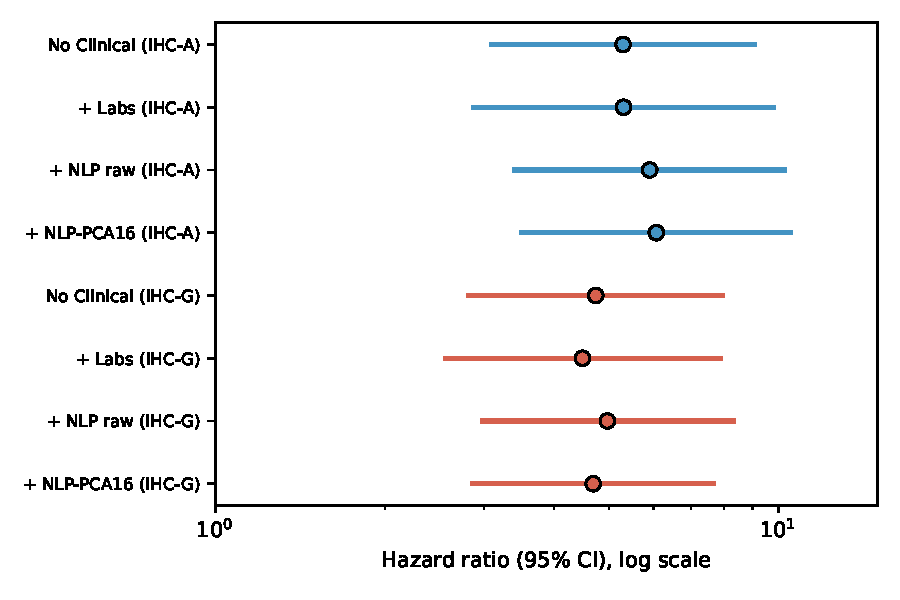
\includegraphics[width=\textwidth]{fig5c_cox_forest.pdf}
    \end{column}
    \begin{column}{0.5\textwidth}
      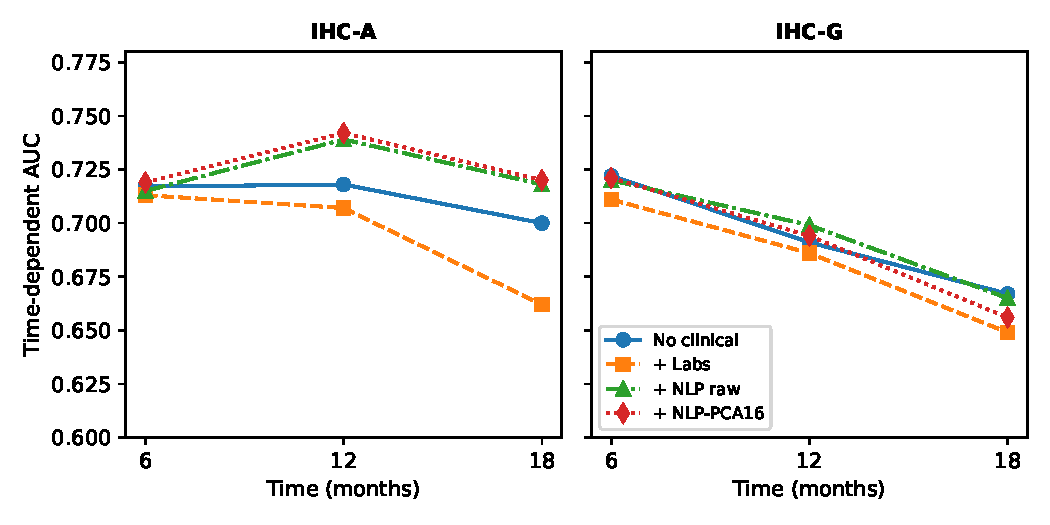
\includegraphics[width=\textwidth]{fig5b_tdauc.pdf}
    \end{column}
  \end{columns}
  \vspace{0.2em}
  \footnotesize
  \begin{itemize}
    \item Risk score DyAM: yếu tố tiên lượng độc lập (Cox $p<0{,}001$, cả 8 biến thể).
    \item \textbf{HR cao nhất luôn thuộc NLP}: 6,07 (IHC-A) / 4,97 (IHC-G) — \alert{số thô KHÔNG cải thiện HR}.
    \item Lợi thế NLP tập trung ở \textbf{12–18 tháng}; Kaplan–Meier tất cả $p<0{,}005$.
  \end{itemize}
\end{frame}

% ── Slide bảng kết quả survival (Table 4 của bài báo + tdAUC) ─────────────────
\begin{frame}{Bảng kết quả phân tích sống còn (8 mô hình)}
  \footnotesize
  \centering
  \begin{tabular}{@{}lcccc@{}}
    \toprule
    \textbf{Mô hình} & \textbf{C-index} & \textbf{Cox HR} & \textbf{tdAUC 12m} & \textbf{IBS}$\downarrow$ \\
    \midrule
    \multicolumn{5}{l}{\textit{Nhánh IHC-A}} \\
    No clinical          & 0,623 & 5,30 & 0,718 & 0,1745 \\
    $+$ Labs             & 0,626 & 5,31 & 0,707 & 0,1739 \\
    $+$ NLP raw          & 0,625 & 5,91 & 0,739 & 0,1723 \\
    \textbf{$+$ NLP-PCA16} & \textbf{0,628} & \textbf{6,07} & \textbf{0,742} & \textbf{0,1716} \\
    \midrule
    \multicolumn{5}{l}{\textit{Nhánh IHC-G}} \\
    No clinical          & 0,626 & 4,74 & 0,691 & 0,1748 \\
    $+$ Labs             & \textbf{0,632} & 4,49 & 0,686 & 0,1746 \\
    \textbf{$+$ NLP raw} & \textbf{0,632} & \textbf{4,97} & \textbf{0,699} & \textbf{0,1736} \\
    $+$ NLP-PCA16        & 0,631 & 4,69 & 0,694 & 0,1736 \\
    \bottomrule
  \end{tabular}

  \vspace{0.5em}
  \begin{columns}[T]
    \begin{column}{0.5\textwidth}
      \scriptsize
      \textbf{\color{vgreen}C-index:} $\approx$0,62–0,63 (đều $\gg$0,5) — nền mạnh; NLP nhỉnh nhẹ, chưa có ý nghĩa.\\[2pt]
      \textbf{\color{vorange}Cox HR:} NLP cao nhất (\textbf{6,07}/4,97); số thô \emph{không} tăng $\rightarrow$ tín hiệu mạnh nhất.
    \end{column}
    \begin{column}{0.5\textwidth}
      \scriptsize
      \textbf{\color{vgreen}tdAUC 12m:} NLP tốt nhất cả 2 nhánh; $+$Labs thấp nhất.\\[2pt]
      \textbf{\color{vorange}IBS:} đều $<0,25$ (hiệu chuẩn tốt); NLP-PCA16 thấp nhất.
    \end{column}
  \end{columns}
  \vspace{0.3em}
  {\scriptsize\textit{Cox đa biến hiệu chỉnh tuổi/ECOG/albumin/dNLR/di căn gan, mọi $p<0{,}001$. In đậm $=$ tốt nhất mỗi cột trong từng nhánh. IBS càng thấp càng tốt.}}
\end{frame}

% ── Slide công thức 1: chỉ số phân biệt ──────────────────────────────────────
\begin{frame}{Chỉ số sống còn (1): Phân biệt --- công thức \& ý nghĩa}
  \small
  \begin{block}{Harrell's C-index --- ``AUC cho dữ liệu sống còn''}
    \[
      C=\frac{\#\{\text{cặp xếp hạng đúng}\}}{\#\{\text{cặp so sánh được}\}}
       = P\!\left(\hat r_i>\hat r_j \mid T_i<T_j\right)
    \]
    Xét mọi \textbf{cặp bệnh nhân} so sánh được $\rightarrow$ tỉ lệ model xếp \textbf{đúng thứ tự nguy cơ}
    (event sớm hơn $\Rightarrow$ risk cao hơn). \;$0{,}5=$ ngẫu nhiên, $1{,}0=$ hoàn hảo.
    CI 95\%: bootstrap 1000 lần. \hfill\textit{(lifelines)}
  \end{block}
  \begin{block}{Time-dependent AUC --- phân biệt tại từng mốc $t$}
    \[
      \mathrm{AUC}(t)=P\!\left(\hat r_i>\hat r_j \mid T_i\le t< T_j\right)
    \]
    Tại $t=6/12/18$ tháng: ``case'' $=$ đã có event trước $t$, ``control'' $=$ còn lại sau $t$;
    hiệu chỉnh kiểm duyệt bằng \textbf{IPCW}. \;Cho biết model mạnh ở \textbf{ngắn hạn hay dài hạn}.
    \hfill\textit{(scikit-survival)}
  \end{block}
  \footnotesize\alert{Trong bài:} $\Delta C=+0{,}005$ (nhất quán, chưa có ý nghĩa); td-AUC: $+0{,}024$@12m, $+0{,}020$@18m.
\end{frame}

% ── Slide công thức 2: hồi quy nguy cơ & hiệu chuẩn ──────────────────────────
\begin{frame}{Chỉ số sống còn (2): Hồi quy nguy cơ \& hiệu chuẩn}
  \scriptsize
  \begin{block}{Cox proportional hazards --- Hazard Ratio (HR)}
    \[
      h(t\mid\mathbf{x})=h_0(t)\,\exp\!\big(\beta_1x_1+\dots+\beta_px_p\big),
      \qquad \mathrm{HR}_{\text{score}}=e^{\beta_{\text{score}}}
    \]
    Đa biến: score (scale $[0,1]$) $+$ tuổi, ECOG, albumin, dNLR, di căn gan.
    \textbf{HR$>$1} $\Rightarrow$ score cao $=$ nguy cơ cao hơn; $p$ (Wald) đo giá trị tiên lượng \textbf{độc lập}.
    \alert{HR $=6{,}07$ vs $5{,}30$ (số thô không cải thiện).}
  \end{block}
  \begin{block}{Integrated Brier Score (IBS) --- hiệu chuẩn}
    \[
      \mathrm{BS}(t)=\frac{1}{N}\sum_i w_i\big(\hat S(t\mid\mathbf{x}_i)-\mathbf{1}\{T_i>t\}\big)^2,
      \quad \mathrm{IBS}=\frac{1}{t_{\max}-t_{\min}}\!\int \mathrm{BS}(t)\,dt
    \]
    Sai số bình phương giữa \textbf{xác suất sống dự đoán} và thực tế (IPCW). Càng thấp càng tốt; $0{,}25=$ ngẫu nhiên.
    \alert{IBS $=0{,}172$–$0{,}175$.}
  \end{block}
  \begin{block}{Kaplan--Meier $+$ log-rank --- phân tầng nguy cơ}
    \[
      \hat S(t)=\!\!\prod_{t_i\le t}\!\Big(1-\frac{d_i}{n_i}\Big),
      \qquad \chi^2_{\text{log-rank}}=\frac{\big(\sum_k(O_k-E_k)\big)^2}{\sum_k \mathrm{Var}(O_k)}
    \]
    Chia 2 nhóm tại score$=0$; log-rank so \textbf{số event quan sát $O_k$ vs kỳ vọng $E_k$}.
    \alert{Mọi $p<0{,}005$; $\chi^2$ cao nhất $=28{,}92$.}
  \end{block}
\end{frame}

% ═══════════════════════════════════════════════════════════════════════════
\section{Bàn luận \& Kết luận}

\begin{frame}{Bàn luận}
  \begin{block}{Vì sao NLP $>$ số thô?}
    Sentence embedding nắm bắt \textbf{tương tác phi tuyến} giữa các biến; bệnh nhân hồ sơ giống nhau $\rightarrow$ vector gần nhau. Số thô buộc mô hình tự học từ tập nhỏ.
  \end{block}
  \begin{block}{Vì sao chưa đạt ý nghĩa thống kê?}
    Giới hạn \textbf{cỡ mẫu}: $n=247 \rightarrow$ CI rộng $\approx\pm0{,}07$; cần \textbf{$\sim$1.200–1.500 BN} để phát hiện $\Delta$AUC$\approx0{,}02$ (power 80\%). Hiệu ứng nhất quán về hướng $\rightarrow$ thật nhưng thiếu power.
  \end{block}
  \begin{block}{Khi nào dùng OvO?}
    Phương thức \textbf{trùng lặp} (ít phương thức) $\rightarrow$ OvO; nhiều phương thức \textbf{bổ sung} $\rightarrow$ cooperative.
  \end{block}
\end{frame}

\begin{frame}{Hạn chế}
  \begin{itemize}
    \item Cohort \textbf{đơn trung tâm, hồi cứu} $\rightarrow$ có thể sai lệch chọn mẫu, hạn chế khái quát hóa.
    \item Cỡ mẫu nhỏ ($n=247$) $\rightarrow$ cải thiện AUC chưa đạt ý nghĩa thống kê.
    \item Sentence encoder dùng \textbf{zero-shot}, chưa fine-tune cho thuật ngữ NSCLC.
    \item PD-L1 chấm theo phương pháp Sauter $\rightarrow$ có thể khác assay SP142/22C3 ở nơi khác.
  \end{itemize}
  \vfill
  \footnotesize\textit{$\Rightarrow$ Định hướng: validation trên cohort lớn, đa trung tâm.}
\end{frame}

\begin{frame}{Kết luận}
  \begin{itemize}
    \item Mở rộng DyAM với \textbf{2 đóng góp}: OvO attention + NLP encoding.
    \item \textbf{OvO:} tốt nhất ở cấu hình ít phương thức; cho mô hình tốt nhất toàn bộ (AUC \alert{0,800}).
    \item \textbf{NLP:} cải thiện AUC ổn định (tới $+0{,}030$) \textbf{và} giá trị tiên lượng độc lập \textbf{mạnh nhất} trong phân tích sống còn.
    \item \textbf{Thực tiễn:} không cần fine-tune; áp dụng cho mọi trường EHR có cấu trúc.
  \end{itemize}
  \vfill
  \begin{alertblock}{Thông điệp}
    Competitive attention + NLP encoding là chiến lược \textbf{thực tế, khái quát hóa được} cho khám phá biomarker đa phương thức. Cần validation đa trung tâm để khẳng định.
  \end{alertblock}
\end{frame}

\begin{frame}[plain]
  \centering
  \vfill
  {\Large\color{vgreen}\textbf{Xin cảm ơn thầy cô và các bạn đã lắng nghe!}}
  \par\vspace{1em}
  {\normalsize Rất mong nhận được câu hỏi và góp ý.}
  \vfill
  {\footnotesize Số liệu chủ chốt: AUC tốt nhất \textbf{0,813} (NLP raw, IHC-G) • \textbf{0,800} (OvO) • HR \textbf{6,07} (NLP-PCA16) • $n=247$.}
  \vfill
\end{frame}

\end{document}
